\begin{figure}[tb]
	\centering
	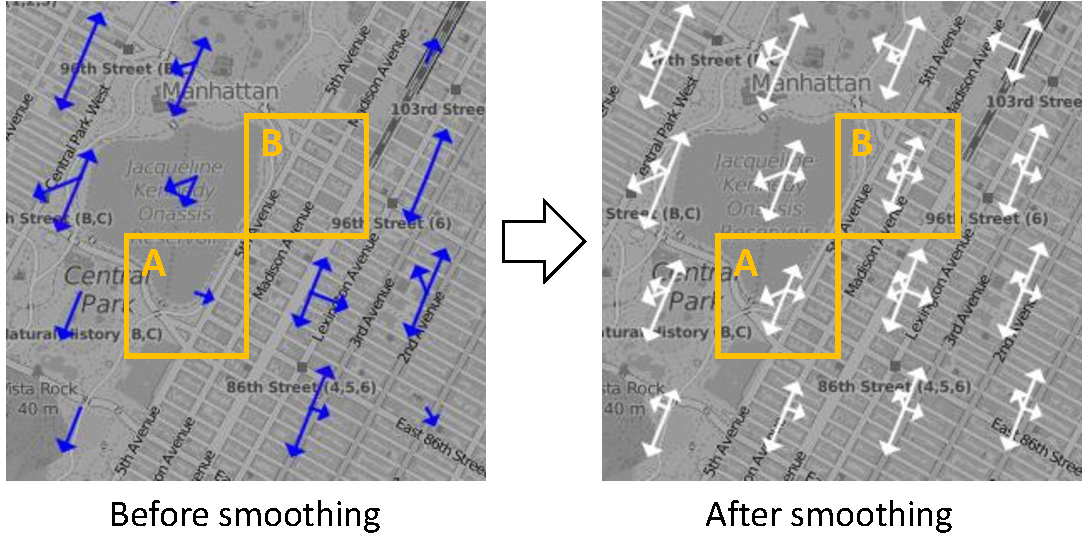
\includegraphics[width=1.0\columnwidth]{smoothdemo}
	\caption{An example of the smoothing result. Sub-space B does not have density due to sparseness data (Left). Sub-space has the density (Right).}
	\label{fig:smoothdemo}
	%\vspace{-0.7cm}
\end{figure}


\begin{figure}[tb]
	\centering
	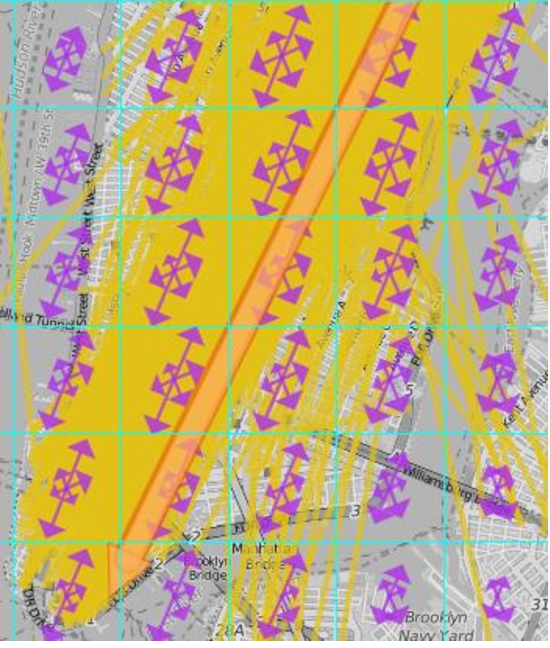
\includegraphics[width=0.6\columnwidth]{nyc_flow}
	\caption{Local directional density (purple arrows) and global (orange arrow) trends of taxi movements in southern Manhattan between 6:00 AM and 10:00 AM.}
	\label{fig:taxi_glyph}
\end{figure}



\section{Flow Data Modeling, Forecasting, and Visualization}

Our flow modeling methodology consists of a pipeline of several processes.
We first apply a directional density estimation technique (Section~\ref{sec:discretization}). 
We then apply a flow smoothing procedure in order to mitigate the data sparseness and noise (Section~\ref{sec:smoothing}).
%At the center of our approach are the methods for computing and smoothing directional density estimation.
After these processes are completed, we forecast the future geospatial flows using the seasonal trend decomposition based on loess technique (Section~\ref{sec:futureflow}) and finally visualize the results using a particle advection technique(Section~\ref{sec:forecasting-visualization}). % and utilize these forecasts the result.
These processes are described in detail in the following sub-sections. 

%AM: I SUGGEST THAT YOU BRING SECTION 4 TO SECTION 3.4.

%We describe these processes in detail below.
%In the next sections, we explain our processing methods and forecasting models to have movement prediction. %First we consider a space over a domain$\Omega\subset \mathbb{R}^{2}$ where a large number of trajectories of a specific time window are projected. Once the data is projected, the given space $\Omega$ are split into multiple sub-spaces $\Omega = \left\{sp_1, \cdots, sp_n\right\}$ in order to estimate and smooth directional density and forecast future flow.
%These methods and models for directional density estimation, smoothing, and forecasting are crucial steps in our computation. We describe those in the next sections in detail. 

%For a given space defined over a domain $\Omega\subset \mathbb{R}^{2}$ in which a large number of trajectories of a specific time window are embedded, we split $\Omega$ into small sub-spaces $\Omega = \left\{sp_1, \cdots, sp_n\right\}$ and estimate the directional density representing the directions of the movements of each sub-space.
%The overall process is illustrated in Figure~\ref{fig:segment}.
%For a given space in which a large number of trajectories are embedded, 
%We discretize the space $\Omega$ through a uniform grid with resolution $R$.
%We discretize the space $SP$ through a uniform grid with cells of a specific size.
%The size depends on the area and the zoom level.
%For each cell, we transform the sub-part of each trajectory passing through the cell boundary into Euclidean vectors.
%For each sub-space $sp_i$, we segment the individual trajectories $tr_i$ passing through the sub-space so each segment is contained on a cell of the grid (see Figure~\ref{fig:segment} (A)).
%Then, we transform the sub-trajectories of $tr_j$ passing through the cell into Euclidean vectors $v_j$ with the same origin point (the center of the cell) (see Figure~\ref{fig:segment} (B)).




%Here is the brief explanation of our forecasting model.
%Our model for forecasting the flow of human crowds consists of the following major steps:
%\begin{enumerate}
%\item embed trajectory data for a time interval into a 2D space, and then, the space is tessellated into square sub-spaces of the same size;
%\item for each sub-space, segment the trajectories so each segment is contained on the sub-space;
%\item transform the trajectory segments into Euclidean vectors and estimate the directional density of the sub-space using the vectors;
%\item smooth the directional density based on local and global directional trends;
%\item create a vector field consisting of location points with representative vectors exhibiting the directional density;
%\item prepare a series of the vector fields for a series of the corresponding past time intervals;
%\item predict the future vector fields for the space based on the series of the past vector fields.
%\end{enumerate}

%The detailed procedure for each step are described in the following sub-sections.

%1) embed trajectory data for a time interval into a 2D space and split the space into discrete grid cells;
%%We discretize the space through a uniform grid with cells of a specific size.
%%The size depends on the area and the zoom level.
%%For each cell, we transform the sub-part of each trajectory passing through the cell boundary into Euclidean vectors.
%2) for each cell, transform the trajectories passing through the cell boundary into Euclidean vectors;
%3) estimate the directional distribution of the vectors in the cell;
%%Then, we summarize the vectors.
%%The traditional methods for the summary of vectors, vector addition, vector average, and spherical linear interpolation have a limitation, which results in a small average vector with a meaningless direction when the directions of the vectors with similar magnitude are evenly distributed.
%%where, our approach is designed as a best-effort method for preserving the original directions of the vectors.
%%We divide one full turn (360\degree) into multiple sectors of a same size and then classify each vector into one of the sectors according to its direction.
%%Each grid cell will have its directional distribution of the trajectories passing the cell (see Figure~\ref{fig:segment} (B)).
%5) smooth the directional distribution based on local and global trends;
%%We adjust the directional distribution of each cell based on the ones of its adjacent neighbor cells and the direction of the global movement around the cell.
%%Individual in a crowd tends to follow dominant paths of the crowd~\cite{Kok:2015:Crowd}.
%6) create a vector field consisting of location points with one or several vectors which are calculated by the directional distribution at each location;
%7) create a series of such vector fields for past time intervals;
%8) predict the future vector fields based on the past vector fields.

%In other words, our model forecasts the future directional distribution of a specific location based on the past ones of the same location using a statistical forecasting technique.
%Then, it repeats the same procedure on each location to create the future vector fields.
%Finally, we visualize the vector fields using particle tracing, a standard flow visualization technique, for representing the future flow of human crowds.

